\chapter{Introduzione}
In questo elaborato andremo ad analizzare come i dati privati vengono utilizzati e qual'è l'importanza nell'adottare politiche di sicurezza in grado di proteggere e preservare tali informazioni all'interno di piattaforme informatiche interconnesse, presentando anche una possibile soluzione che possa essere di uso ottimale in casi particolari. Nel capitolo introduttivo, andremo a soffermarci sulla situazione del contesto attuale, specificando l'uso e la protezione dei dati in rete per poi analizzare quali siano le conseguenze nell'adattabilità alla GDPR. 
\section{Utilizzo dei dati privati su Internet}
Internet, la rete delle reti, è un magazzino di dati costantemente in crescita. I dati che vi sono al suo interno sono le fondamenta delle funzionalità dei servizi che compongono le piattaforme accessibili in rete. Un'esempio lo possiamo vedere con Amazon, un colosso nel commercio elettronico che, nell'ultimo decennio, ha raggiunto il primato nel commercio online grazie anche a politiche di gestione dei dati interne basate sui cookie privati che, grazie al loro utilizzo, sono riusciti ad ottimizzare funzionalità come il tenere traccia delle proprie preferenze, dei prodotti nel carrello, oppure nella gestione dei suggerimenti in modo da garantire un meccanismo pubblicitario che, sotto un punto di vista del marketing elettronico, dovrebbe aumentare la possibilità di effettuare un'acquisto. L'utilizzo dei dati privati non si limita solamente ai fini commerciali, ma vi sono usi anche all'interno dell'ambito sanitario, industriale e bancario. 
In conclusione, possiamo dire che una delle colonne portanti dei servizi tecnologici odierni è rappresentato dai dati. Per cui, bisogna sempre garantire meccanismi di sicurezza in grado di poter evitare un uso improprio delle informazioni che si ricevono in ingresso cosi da poter garantire affidabilità nelle attività proposte. 
\section{Criteri di affidabilità dei servizi contro i cyber-crime}
L'affidabilità di un servizio si può garantire andando a definire delle politiche di sicurezza basate su tre caratteristiche principali:
\begin{itemize}
    \item Disponibilità dei dati: ossia salvaguardia del patrimonio informativo nella garanzia di accesso, usabilità e confidenzialità dei dati. Da un punto di vista di gestione della sicurezza significa ridurre a livelli accettabili i rischi connessi all’accesso alle informazioni come intrusioni e furto di dati.
    \item Integrità dei dati: intesa come garanzia che l’informazione non subisca modifiche o cancellazioni a seguito di errori o di azioni volontarie, ma anche a seguito di malfunzionamenti o danni dei sistemi tecnologici.
    \item Riservatezza informatica: cioè gestione della sicurezza in modo tale da mitigare i rischi connessi all’accesso o all’uso delle informazioni in forma non autorizzata e ovviamente data privacy.
\end{itemize}

Tali criteri risultano alla base della qualità di un servizio, soprattutto negli ultimi anni in cui, secondo i rapporti Clusit del 2019 , nel biennio scorso il tasso di crescita del numero di attacchi gravi è aumentato di 10 volte rispetto al precedente. Non solo, la Severity media di questi attacchi è contestualmente peggiorata, agendo da moltiplicatore dei danni. Sotto un punto di vista statistico, gli attacchi informatici gravi annui fino alla fine del 2018 sono pari a 1552 (+37.7\% rispetto l'anno precedente) con una media mensile di 129 attacchi al mese (rispetto ai 94 mensili del 2017 e 88 negli ultimi 8 anni).

\begin{figure}[h]
    \centering
    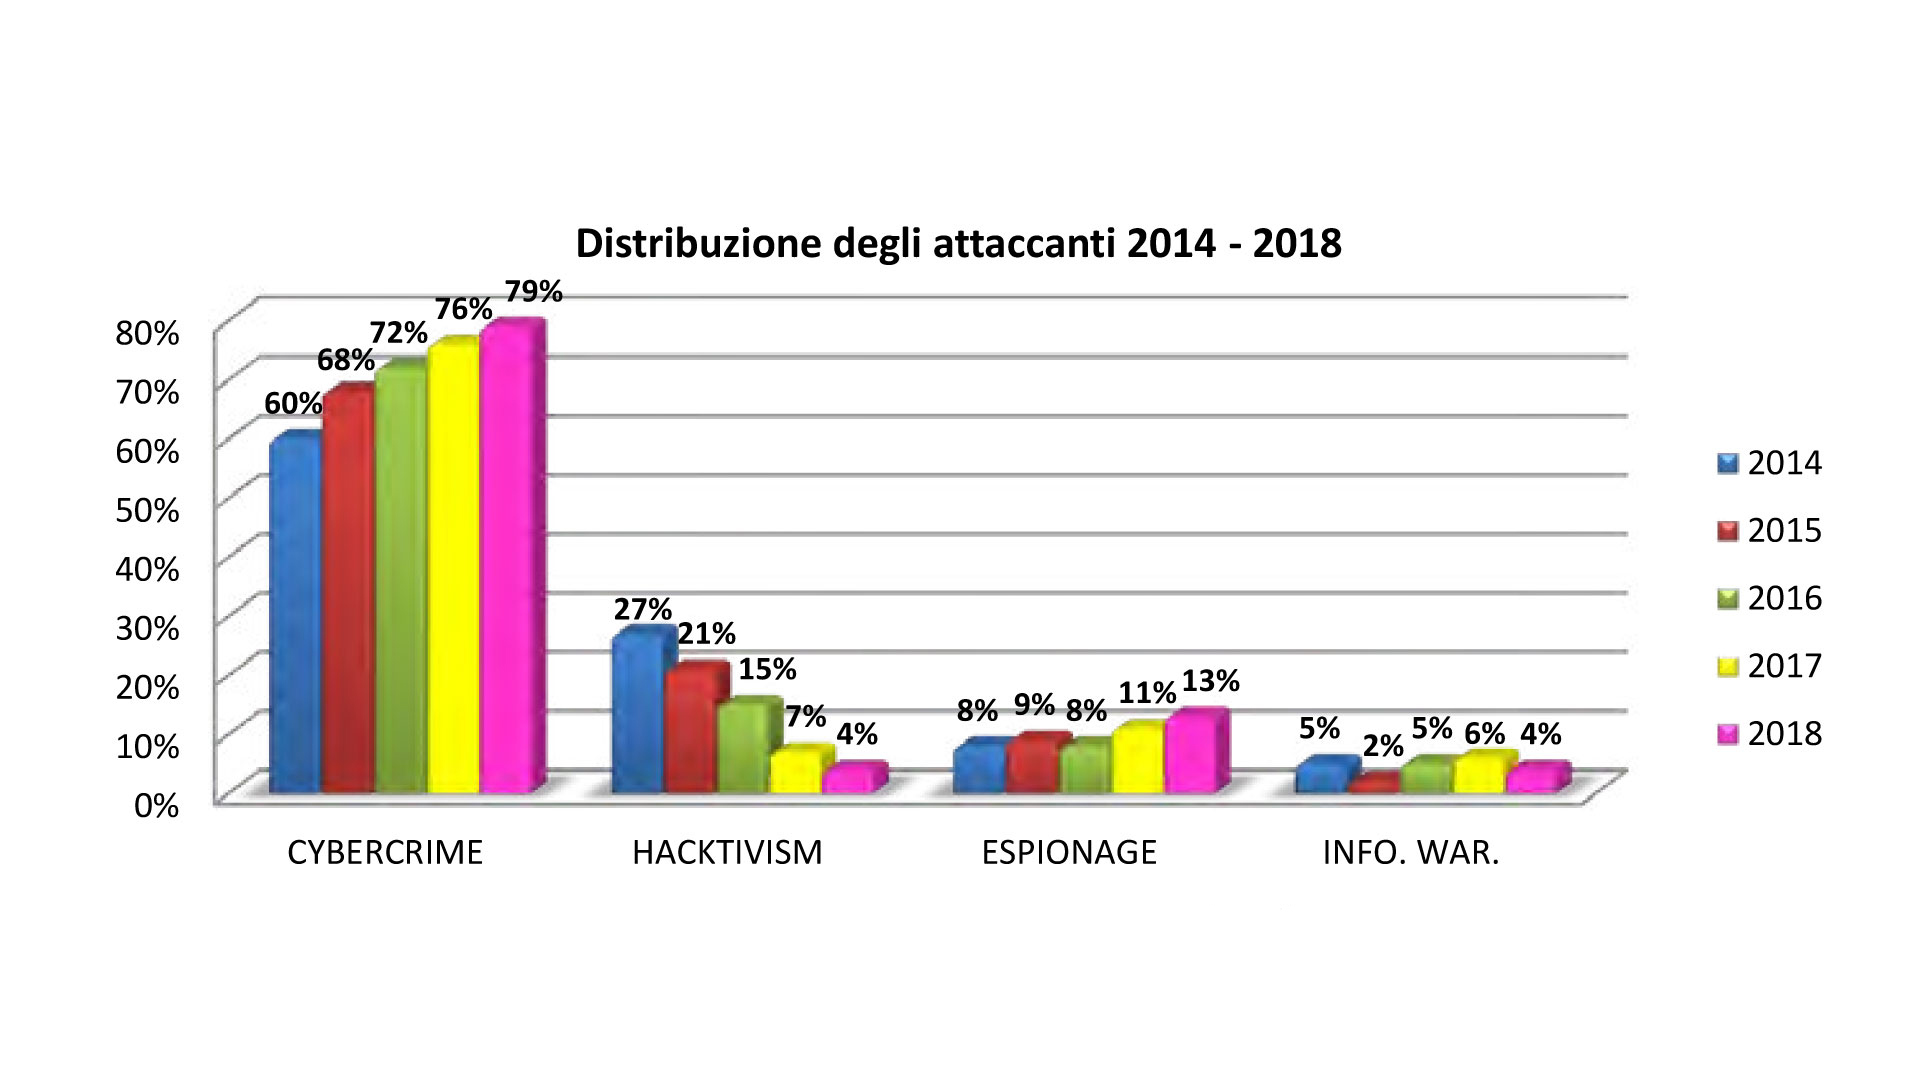
\includegraphics[width=0.8\textwidth]{img/clusit.jpg}
    \caption{Rapporto di distribuzione degli attacchi in ambito ICT in Italia}
    \label{fig:clusit}
\end{figure}

Tali risultati hanno portato all'incremento degli investimenti per aumentare la protezione dei dati e, in generale, rendere i servizi più sicuri. Anche se gli investimenti sono sufficienti, bisogna sempre dover stabilire una infrastruttura di sicurezza che sia efficiente il più possibile per poter preservare i dati in maniera più sicura e trasparente. A ciò, bisogna anche aggiungere anche i costi relativo all'adattamento delle piattaforme verso i criteri di gestione dei dati privati dettati dalla GDPR (General Data Protection Regulator) attiva dal 25 Maggio 2018. 

\newpage
\section{Adattabilità alla GDPR}
La GDPR  è la nuova normativa per la gestione dei dati sensibili e privati propri di un cittadino europeo da parte di aziende private o pubbliche anche se non residenti su suolo europeo. I criteri che riguardano il nuovo regolamento aumentano gli obblighi del titolare del trattamento per garantire la tutela dei dati e i diritti del soggetto interessato. I due aspetti fondamentali sono:

\begin{itemize}
    \item Privacy by design: sin dall'inizio del progetto, bisogna stabilire le misure e le procedure adeguate per garantire la tutela dei dati trattati.
    \item Privacy by default: i dati devono essere trattati con la massima chiarezza, indicando le finalità, le modalità e la durata del trattamento degli stessi.
\end{itemize}

Alla base di tale normativa, vi è l'esplicitazione nell'utilizzo dei dati privati e sotto quali finalità vengono utilizzati, andando ad adottare una politica di gestione il più trasparente possibile. Inoltre, si devono gestire solamente i dati essenziali, ossia si devono raccogliere solamente quei dati che vengono realmente utilizzati all'interno dei servizi offerti, andando a gestirne anche l'aggiornamento in modo da garantire in qualsiasi istante la correttezza. Infine, bisogna tenere un sistema di archiviazione basato sul mantenimento delle informazioni utilizzate recentemente in qualche servizio, rimuovendo tutti i dati obsoleti e non più utili all'interno della piattaforma in cui sono stati utilizzati. 

L'adattabilità a tali requisiti ha portato la diffusione di architetture ICT che si basano sulla trasparenza, sicurezza e la correttezza dei dati. Una delle possibili soluzioni è quella basata sulle tecnologie blockchain che, seguendo il modello private o permissioned, adottano una politica di gestione e archiviazione di dati nel pieno rispetto della GDPR.

\newpage